
% !TEX TS-program = pdflatex
% !TEX encoding = UTF-8 Unicode

% This is a simple template for a LaTeX document using the "article" class.
% See "book", "report", "letter" for other types of document.

\documentclass[11pt]{article} % use larger type; default would be 10pt

\usepackage[utf8]{inputenc} % set input encoding (not needed with XeLaTeX)

%%% Examples of Article customizations
% These packages are optional, depending whether you want the features they provide.
% See the LaTeX Companion or other references for full information.

%%% PAGE DIMENSIONS
\usepackage{geometry} % to change the page dimensions
\geometry{a4paper} % or letterpaper (US) or a5paper or....
% \geometry{margin=2in} % for example, change the margins to 2 inches all round
% \geometry{landscape} % set up the page for landscape
%   read geometry.pdf for detailed page layout information

\usepackage{graphicx} % support the \includegraphics command and options

% \usepackage[parfill]{parskip} % Activate to begin paragraphs with an empty line rather than an indent

%%% PACKAGES
\usepackage{booktabs} % for much better looking tables
\usepackage{array} % for better arrays (eg matrices) in maths
\usepackage{paralist} % very flexible & customisable lists (eg. enumerate/itemize, etc.)
\usepackage{verbatim} % adds environment for commenting out blocks of text & for better verbatim
\usepackage{subfig} % make it possible to include more than one captioned figure/table in a single float
% These packages are all incorporated in the memoir class to one degree or another...

%%% HEADERS & FOOTERS
\usepackage{fancyhdr} % This should be set AFTER setting up the page geometry
\pagestyle{fancy} % options: empty , plain , fancy
\renewcommand{\headrulewidth}{0pt} % customise the layout...
\lhead{}\chead{}\rhead{}
\lfoot{}\cfoot{\thepage}\rfoot{}

%%% SECTION TITLE APPEARANCE
\usepackage{sectsty}
\allsectionsfont{\sffamily\mdseries\upshape} % (See the fntguide.pdf for font help)
% (This matches ConTeXt defaults)

%%% ToC (table of contents) APPEARANCE
\usepackage[nottoc,notlof,notlot]{tocbibind} % Put the bibliography in the ToC
\usepackage[titles,subfigure]{tocloft} % Alter the style of the Table of Contents
\renewcommand{\cftsecfont}{\rmfamily\mdseries\upshape}
\renewcommand{\cftsecpagefont}{\rmfamily\mdseries\upshape} % No bold!

\makeatletter
   \newcommand\figcaption{\def\@captype{figure}\caption}
   \newcommand\tabcaption{\def\@captype{table}\caption}
\makeatother
%%% END Article customizations

%%% The "real" document content comes below...

\title{CSE 524 Project Report}
\author{Arun Rathakrishnan}
%\date{} % Activate to display a given date or no date (if empty),
         % otherwise the current date is printed 

\begin{document}
\maketitle

\section{Introduction}
Given a set of points in a two plane, $R \times R$ in set $S$, we attempt to
find a "good" ordering $P$ of points in $S$. Let $c_i$ be, the center of mass
of $P$ after the $i^{th}$ point is placed. Some definitions of good are,
ordering points in $P$ such that the interval of $c_i$ is minimized or the
total distance $c_i$ moves as each point is placed, is minimized. These are the
two factors considered for evaluating any ordering in this project. For
measuring the interval, we consider the area of the convex hull of set of
points from $c_0$ to $c_{n-1}$.  We also consider a variant of the problem
where we are allowed to pick at most $k$ points to be placed in set $P$ at a
time, instead of exactly one in the original problem description.  

\section{Heuristics}
We have compared $5$ heuristics during the test runs.
\begin{description}
\item [Greedy Range Minimization (H1)] Keep $c_i$ closest to $c_n$, picking one point
at a time. It aims to minimize the area of the convex hull enclosing the set of
points formed by $c_i$.
\item [Greedy Movement Minimization (H2)] Keep $c_i$ closest to $c_{i-1}$, picking one
point a time. Greedily tries to minimize the total movement of $c_i$.
\item [Greedy Range Minimization (Two simultaneous selections -H3)] Pick two points
at a time such that $c_i$ after picking two points at the $i^{th}$ attempt is
closest to $c_n$.
\item [Greedy Movement Minimization (Two simultaneous selections -H4)] Pick two point
at a time such that, the center of mass after the $i^{th}$ attempt $c_{i-1}$ is
closest to $c_i$.
\item [Greedy Balancing Pair (Two simultaneous selections -H5)]: Pick two points at a
time such that their average is closest to $c_n$.
\end{description}

\section{Results}
 For the experiment we randomly generated points in $R \times R$. In each case
 the range (interval) or the movement of center of mass  is compared with
 respect to the corresponding optimal value. If input points are collinear, the
 $2D$ heuristics for the interval do not apply, as the area of the convex hull of
 midpoints is $0$ for any ordering points. But, we can identify such cases and
 run $1D$ heuristics on them instead of $2D$ heuristics.  If the center of
 masses of a set of points happens to be collinear in a selection, we have no
 means to compare the result with other arrangement of points, which are not
 collinear.\\

 The figure below shows the comparison of the interval of center of mass with
 respect to the optimal value.  Greedy Range Minimization Heuristic (H1)
 performs better than other heuristics. Though the interval value from H1 is always
 within two times the optimal value for all test runs for $1D$ case, for $2D$ case,
 there are some inputs for which the ratio is above $4.0$.  For heuristics that
 pick 2 points at a time, we evaluate range/interval value for Fig 1. as if the
 pair of points were picked one after the other.
 \\
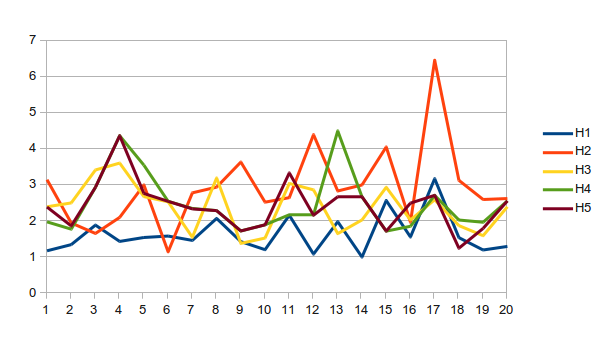
\includegraphics{result0.png}
\begin{center}
\caption{Fig 1. Interval of Center of Mass}
\end{center}
\\
 In Fig 2. we evaluate the movement of center of mass, where Greedy Movement
 Minimization (H2) performs the best. As in the $1D$ case, the approximation
 ratio remained below $2.0$ during all test runs.
\\
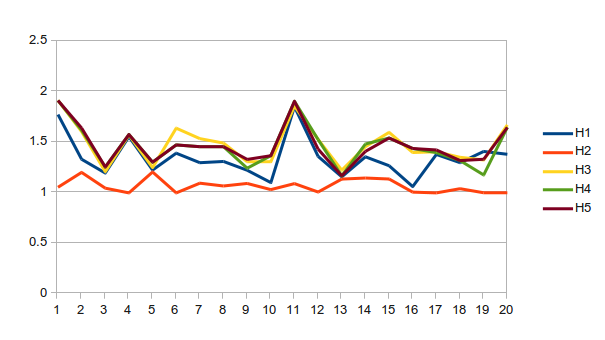
\includegraphics{result1.png}
\begin{center}
\caption{Fig 2. Movement of Center of Mass}
\end{center}
\\
Similar to the $1D$ analysis, comparisons of H3, H4 and H5 heuristics when we consider both
the points are placed simultaneously to the performance of H1 and H2 was considered. For the
two dimensional case, simultaneous selections proved more effective than H1 and H2.

\pagebreak
\\
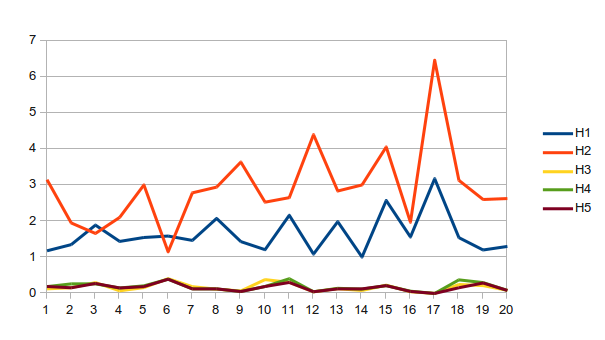
\includegraphics{result2.png}
\begin{center}
\caption{Fig 3. Interval of Center of Mass Simultaneous Selection}
\end{center}
\\
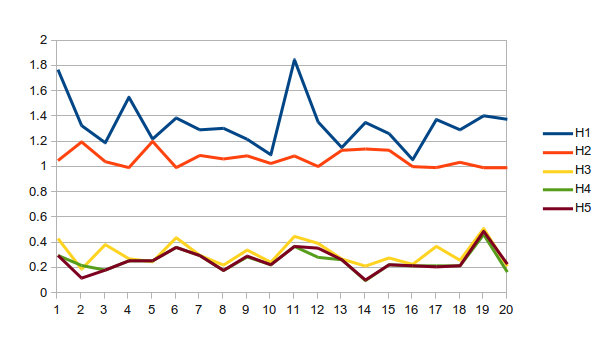
\includegraphics{result3.png}
\begin{center}
\caption{Fig 4. Movement of Center of Mass Simultaneous Selection}
\end{center}
\end{document}
